\documentclass[headsepline=true, footsepline=true]{scrartcl}

\usepackage{tutorial}

% % ==============================================================
\title{Separates Deployment von Produktdaten}
\author{Cornelius Dirmeier}
\setcopyright{
\includegraphics[height=10pt]{./pics/FaktorZehn-ORG.png}}
% % ==============================================================

\begin{document}

\maketitle

\section{Einleitung}

Faktor-IPS verwaltet Produktdaten während der Produktentwicklung in XML Dateien.
Zur Laufzeit liegen die Produktdaten in XML-Ressourcen vor, Formeln werden in
Java-Klassen generiert. Die XML-Ressourcen werden meist in Bibliotheken (z.B.
JAR-Dateien) zusammengefasst werden. Um die Produktdaten zu laden müssen sie zur Laufzeit im Classpath der
Applikation verfügbar sein. Innerhalb einer Applikation kann auf die Produktdaten über ein
Runtime Repository (z.B. $ClassloaderRuntimeRepository$) zugegriffen werden.
Diese Aufteilung wird in Abbildung \ref{old_architecture} verdeutlicht. 

\begin{figure}[htb] \centering
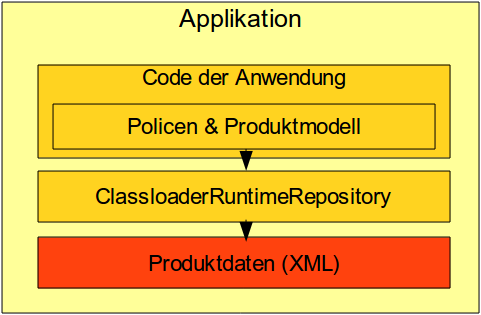
\includegraphics[width=8cm]{./pics/old_architecture.png} \caption{Bisher wurden
Programmcode und Produktdaten in einer gemeinsamen Applikation ausgeliefert}
\label{old_architecture}
\end{figure}

Da sowohl Programmcode als auch Produktdaten als Dateien vorliegen, können sie
zusammen in einem Werkzeug wie CVS oder Subversion gespeichert werden. Eine
fertige Version von Programmcode und Produktdaten wird dann in eine Zielumgebung
transportiert. Im JavaEE Umfeld wird dazu ein Enterprise Archive (EAR) bzw. ein
Web Application Archive (WAR) erzeugt.

Werden die Produktdaten verändert oder erweitert muss dieses Archiv ausgetauscht
werden. Da Produktdaten und Programmcode eine Einheit bilden, muss auch der
Programmcode neu ausgeliefert werden.

Ziel des separaten Deployments von Produktdaten ist es, bei einer Änderung der
Produktdaten nur die XML-Ressourcen auszutauschen ohne den Programmcode neu
ausliefern zu müssen. Die dabei auftretenden Herausforderungen und die daraus
entwickelten Lösungen werden in diesem Dokument vorgestellt.

\section{Herausforderungen}

In diesem Kapitel werden die Probleme, die sich auf dem Weg zum getrennten
Deployment von Produktdaten ergaben aufgezeigt. Im Kapitel
\ref{loesungen} wird zu jedem Problem die entwickelte Lösung präsentiert.

\subsection{Runtime Repository}

Für den Zugriff auf die Produktdaten steht in Faktor-IPS zur Laufzeit das
Interface $IRuntimeRepository$ zur Verfügung. Wie bereits einleitend erwähnt
wird meist die Implementierung $ClassloaderRuntimeRepository$ verwendet.
Dieses lädt die Produktdaten über den Klassenpfad als Ressourcen.

Um die Produktdaten unabhängig vom Programmcode zu halten muss zunächst ein
Repository entwickelt werden, dass die Produktdaten unabhängig vom Klassenpfad
der Applikation laden kann. Die später vorgestellte Lösung greift dazu
auf einen J2EE Service (EJB 3.0 Stateless Session Bean) zu; die Verwendung
einer Datenbank ist ohne großen Aufwand möglich.

\subsection{Ausführen von Formeln}

In Faktor-IPS ist es möglich Formeln in einer einfachen Formelsprache in einem
Produktbaustein einzugeben. In den Modellklassen wird lediglich die Signatur der
Formel festgelegt, die Berechnungsvorschriften liegen in den Produktdaten. Um
diese Formeln zur Laufzeit auszuführen werden sie vom Faktor-IPS-Builder in
Java-Code übersetzt.

Dazu wird für jede Anpassungsstufe eines Produktbausteins eine Subklasse
erzeugt in der die Methode der Formel überschrieben wird. Das Runtime Repository
ist so aufgebaut, dass es jeweils die korrekte Implementierung zu einem
Produktbaustein lädt.

\begin{figure}[htb] \centering
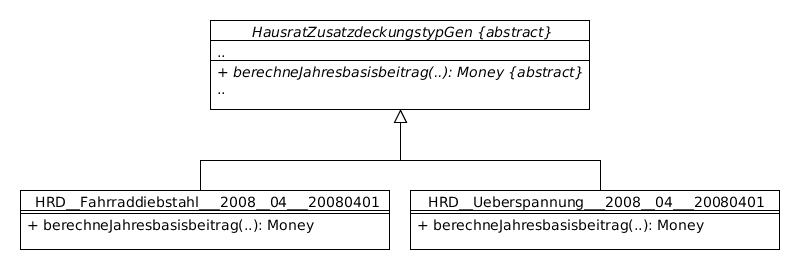
\includegraphics[width=13cm]{./pics/subclassing.png} \caption{Für jeden
Produktbaustein wird eine Subclass angelegt, in der die übersetzte Formel
implementiert ist (Beispiel aus Faktor-IPS Tutorial Teil
2)}
\label{subclassing}
\end{figure}

Werden nun die Produktdaten durch einen separaten Service abgerufen, muss nach
diesem Ansatz auch die Implementierung über den Service abgerufen werden. Ändert
sich in einer neuen Version der Produktdaten eine Formel, muss auch die
Implementierung ausgetauscht werden. Der Classloader von Java sieht jedoch keinen
Austausch von Klassen während des Betriebs vor. Anpassungen am Classloader sind
im J2EE Umfeld durch die EJB Spezifikation verboten.

Eine Herausforderung im separaten Deployment ist es daher, die Formeln nicht wie
bisher in Subklassen zu kompilieren sondern zur Laufzeit zu interpretieren. Die
Produktdaten werden dadurch frei von Programmcode.

\subsection{Konsistenter Zustand der Daten während einer Anfrage}
\label{requests}

Mit dem Separaten Deployment von Produktdaten soll es möglich sein, ohne
Unterbrechung der Anwendung neue Produktdaten auszuliefern. Im Fall
eines EJB Services wird also der Service, der die Produktdaten bereitstellt, per
Hot-Deployment ausgetauscht.

Nehmen wir an, ein Client\footnote{Als Client bezeichnen wir ein Programm, das
Produktdaten abruft - also der Client des Runtime Repositories} möchte
Produktdaten verarbeiten. Dazu muss er im Allgemeinen eine Reihe von Anfragen an
das Repository senden: z.B. fordert der Client einen Produktbaustein an, dann die
aktuell gültige Generation und daraufhin alle assoziierten Produktbausteine. Für
den Client ist dabei wichtig, dass er innerhalb seiner Anfrage auf einem
konsistenten Datenstand arbeitet. Im Beispiel in Abbildung
\ref{concurrent_access} wurden vom $Client 1$ bereits die Produktdaten $P1$ und
$D1$ geladen. Dann wurden die Produktdaten ausgetauscht. Ruft der Client nun das
Objekt $D2$ ab, muss darauf geachtet werden, dass er nicht das neue
Objekt $D2'$ erhält. Das Repository muss entweder in der Lage sein, weiterhin
die alten Daten auszuliefern (z.B. wenn die Daten noch im Cache liegen) oder eine
Exception werfen, damit der Client die Abfrage abbricht.

\begin{figure}[htb] \centering
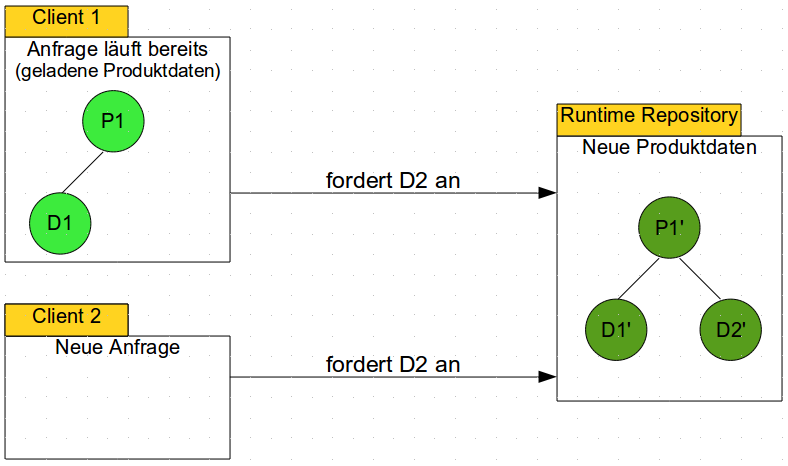
\includegraphics[width=13cm]{./pics/concurrent_access.png} \caption{Während der
Anfrage von Client 1 wurden die Produktdaten ausgetauscht. Client 1 muss eine
Exception erhalten, Client 2 kann mit den neuen Daten arbeiten}
\label{concurrent_access}
\end{figure}

$Client 2$ beginnt dagegen seine Anfrage erst nachdem die Produktdaten
ausgetauscht wurden. Für ihn soll es kein Problem sein, das Objekt $D2$
anzufordern. Das Runtime Repository muss daher wissen, welche Clients bereits
mit den neuen Daten arbeiten und welche auf dem alten Stand sind.

\section{Lösungen}
\label{loesungen}

\subsection{Überblick der Architektur}

Um die im folgenden vorgestellte Lösung zu verwenden, werden
die Runtime Addons\footnote{Dateiname des Archivs:
faktorips-runtime-addons-[version].zip} von Faktor-IPS beötigt. Das Archiv kann
über die Download-Site\footnote{http://update.faktorzehn.org/faktorips/cgi/download.pl?subfolder=v3} heruntergeladen werden.

Wie bereits in der Einleitung erwähnt, betrachten wir die Auslieferung in einem
Java EE Umfeld. Die verschiedenen Programmteile werden als Services implementiert
und in einem EAR ausgeliefert.

Wie bisher wird der Programmcode mit den Modellklassen in einem Archiv gekapselt.
Anstatt des $ClassloaderRuntimeRepositorie$s wird eine neue Implementierung des
Interfaces $IRuntimeRepository$ verwendet: das
$DerivedContentRuntimeRepository$. Dieses ruft zum Laden der Produktdaten einen separaten Service auf, den
Product-Data-Service. Im Klassenpfad des Product-Data-Service sind die
Produktdaten weiterhin als XML-Ressourcen enthalten und können vom Service als
Ressourcen geladen werden.

\begin{figure}[htb] \centering
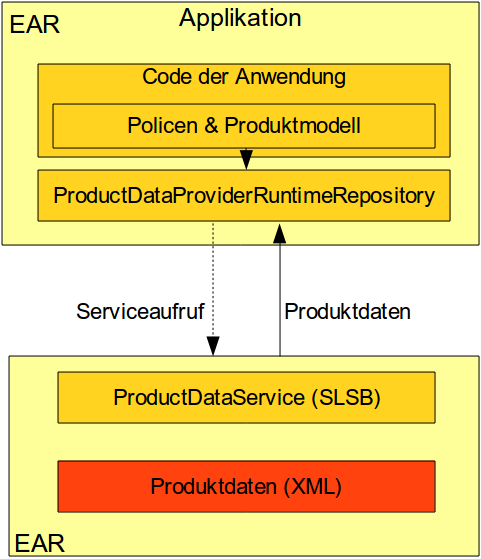
\includegraphics[width=8cm]{./pics/service_architecture.png} \caption{Die
Produktdaten werden in einem separaten Service ausgeliefert der vom Runtime
Repository verwendet wird}
\label{service_architecture}
\end{figure}

Der Product-Data-Service wird als Stateless Session Bean (SLSB) implementiert.
Die Produktdaten werden als XML-Ressourcen geladen, der Inhalt wird an das
Runtime Repository übergeben. Die Instantiierung findet weiterhin im Runtime
Repository statt.

\subsection{Interpretation von Formeln}

Anstatt die Formeln als Java-Code in Subklassen zu generieren kann der
Java-Code der übersetzten Formel ab Version 3.0 auch direkt in die XML Dateien
der Produktdaten geschrieben werden. Diese Option wird in den Einstellungen für den Faktor-IPS Code Generator
unter der Option "`Formula Compiling"' eingestellt. Als Standard wird der
Java-Code sowohl in Subklassen als auch in das XML geschrieben - zur Laufzeit
kann damit sowohl das alte als auch das neue Runtime Repository verwendet
werden.

Zur Laufzeit wird der Java-Code aus den XML-Dateien gelesen und von
Groovy\footnote{http://groovy.codehaus.org/, Version 1.6.0} ausgeführt. Die
Produktdaten enthalten dadurch keinen Programmcode und sind unabhängig vom Classloader der
Applikation.

\subsection{Konsistenter Zustand der Daten während einer Anfrage}

Um innerhalb einer Anfrage einen konsistenten Datenstand zu gewährleisten, ist es
notwendig, dass ein Client den Beginn seiner Anfrage ankündigt. Nach dem
optimistischen Locking Verfahren kann die Anfrage abgearbeitet werden, bis es zu
einem Fehler kommt. Wenn ein Fehler auftritt muss die Anfrage verworfen und
evtl. neu gestartet werden. Da der Austausch von Produktdaten nicht besonders
oft auftritt, ist das optimistische Locking Verfahren völlig ausreichend.

Um dieses Locking zu realisieren wird ein Runtime Repository Manager eingeführt.
Jeder Client erhält zunächst anstatt des Runtime Reposiories einen Manager.
Möchte ein Client eine neue Anfrage starteten, ruft er die Methode
$getActualRuntimeRepository()$ am Manager auf. Der Manager liefert daraufhin ein
Runtime Repository mit dem der Client auf den aktuell gültigen Produktdaten
arbeiten kann. Vor der nächsten Anfrage holt sich der Client erneut das aktuelle
Repository. Haben sich die Produktdaten nicht geändert, wird das gleiche
Repository zurück gegeben. Dieser Ablauf ist im Sequenzdiagramm in
Abbildung \ref{clientSequenceEasy} abgebildet.

\begin{figure}[htb] \centering
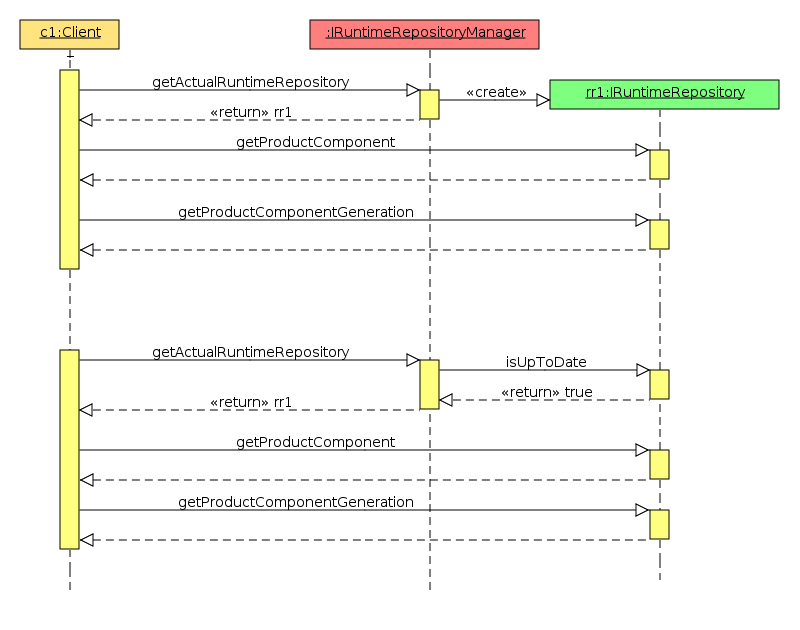
\includegraphics[width=13cm]{./pics/clientSequenceEasy.png} \caption{Der Client
holt sich vor Beginn einer Anfrage das aktuelle Runtime Repository; solange sich
keine Daten ändern arbeitet er auf dem gleichen Repository weiter.}
\label{clientSequenceEasy}
\end{figure}

Werden während der Anfrage die Produktdaten ausgetauscht wirft das Runtime
Repository beim nächsten Abruf von
Produktdaten eine $DataModifiedRuntimeException$. Der Client muss
daraufhin seine Anfrage verwerfen.

Um eine neue Anfrage mit geänderten Produktdaten zu starten wird vom Manager ein
neues Repository geholt. Der Manager stellt die geänderten Produktdaten
fest und erzezgt ein neues Runtime Repository. Der Client arbeitet nun auf
den neuen Produktdaten. Dieses Verhalten ist
im Sequenzdiagramm in Abbildung \ref{clientSequenceChange} dargestellt.

\begin{figure}[htb] \centering
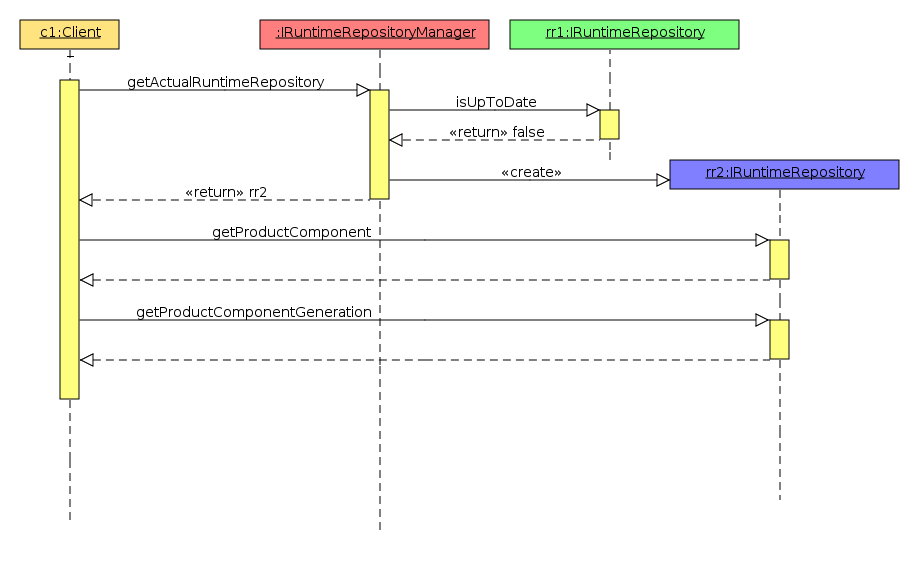
\includegraphics[width=\textwidth]{./pics/clientSequenceChange.png} \caption{Der
Manager stellt fest, dass sich die Produktdaten geändert haben und erstellt ein
neues Runtime Repository}
\label{clientSequenceChange}
\end{figure}

Um die Performance der Abfragen zu erhöhen, enthalten Runtime Repositories einen
Cache und speichern darin bereits abgefragte Produktdaten. Um die Zahl der
Abbrüche beim Austausch von Produktdaten weiter zu verringern wurde das Runtime
Repository so entwickelt, dass es nur beim Abruf von nicht gespeicherten
Produktdaten einen Fehler wirft - solange der Client nur auf Produktdaten im
Cache zugreift, kann er dadurch seine Anfrage zu ende führen.

Auch der gleichzeitige Zugriff mehrerer Client ist mit dieser Lösung kein
Problem. Lediglich der Abruf des aktuellen Runtime Repositories und der gemeinsam
genutzte Cache müssen Threadsicher implementiert werden.

In der Client-Implementierung ist es sinnvoll, einen Manager an zentraler Stelle
zu konfigurieren, damit alle Clients auf den gleichen Manager zugreifen. Zur
Instantiierung des $DetachedContentRuntimeRepositoryManager$ wird ein
Builder\footnote{Dieser Builder ist nach Item 2 im Buch "`Effective Java"' von
Joshua Bloch \cite{effectiveJava} erstellt und weicht vom bekannten Builder
Design Pattern ab.} verwendet. Der Builder ist als innere Klasse des
Repository Managers realisiert und erwartet eine Implementierung von
$IProductDataProviderFactory$ zum instantiieren des Product-Data-Providers.
Optional kann man im Builder weitere Voreinstellungen treffen. Insbesondere eine Implementierung von $IFormulaEvaluatorFactory$\footnote{z.B.
GroovyFormulaEvaluatorFactory zur Ausführen der Formeln mit Groovy (in den
Addons enthalten)} zum ausführen der Formeln sollte gesetzt werden. Ist der
Builder fertig konfiguriert, wird die Methode $build()$ aufgerufen - als Ergebnis erhält man einen $DetachedContentRuntimeRepositoryManager$. 
Ein Beispiel zur Instantiierung des Managers wird im Kapitel \ref{appExample}
gegeben.

\subsection{Verknüpfen mehrerer Repositories}

In den meisten Fällen werden Modell- und Produktdaten in mehrere Projekte
untergliedert. Für den Zugriff auf die Daten muss zur Laufzeit für jedes dieser
Projekte ein eigenes Runtime Repository instantiiert werden.
Analog zu den Referenzen zwischen den Projekten müssen auch dei Runtime
Repositories miteinander verbunden werden, um mit einer Abfrage an alle
relevanten Daten zu gelangen.

Mit der Einführung des Runtime Repository Managers ist es nun Aufgabe des
Managers neue Repositories zu erstellen. Es muss damit ebenfalls sichergestellt
werden, dass in einem neuen Repository alle notwendigen Verknüpfungen gesetzt
sind. Da sich auch in verknüpften Repositories Produktdaten ändern können, muss
der Manager außerdem überprüfen, ob sich in einem referenzierten Repository die
Daten geändert haben.

Um diese Aufgaben zu bewältigen werden die Manager analog zu den Runtime
Repositories miteinander verknüpft. Ein Manager kann dadurch alle verbundenen
Manager nach dem aktuellen Repository fragen und entsprechend das eigene
Repository zusammen bauen.

\subsection{Beispiel einer Applikation}

Das folgende Beispiel baut auf den Tutorial Projekten auf. Der Programmcode der
Tutorial Projekte kann von http://faktorzehn.org/fips:tutorial runtergeladen
werden. 

Die Implementierung des hier vorgestellten Beispiels kann ebenfall
von der Turorial Site runter geladen werden.
Der Product Data Service sowie der EJB Product Data Provider liegen auch im Runtime Addons Archiv
im Faktor IPS
Downloadbereich\footnote{http://update.faktorzehn.org/faktorips/cgi/download.pl?subfolder=v3} bereit.

\subsubsection{Beispiel für den ProductDataService}

Um das neue Runtime Repository zu testen benötigen wir zunächst einen
Application Server, in dem der $ProductDataService$ laufen kann. Im
Projekt ProductDataServiceDemo wird dazu der Apache
OpenEJB\footnote{http://openejb.apache.org} Server verwendet. 
Der Server wird über die Launch-Konfiguration $ProductDataServiceDemo (OpenEJB
Server)$ gestartet. Die Konfiguration liegt im Projekt
$org.faktorips.tutorial.de.ProductDataServiceDemo$.
Der OpenEJB Server packt automatisch alle Bibliotheken im Classpath und deployd
darin enthaltene Services. Im Klassenpfad sind neben dem ProductDataService auch die Produktdaten
des Tutorialprojekts $Hausratproduk$ enthalten.

Konfiguriert wird der Service im Deployment Descriptor in der Datei
$ejb-jar.xml$. Im Listing \ref{ejb-jar.xml} ist die Konfiguration aus dem
Beispiel abgebildet. Darin wird der Service
$org.faktorips.tutorial.ProductDataServiceDemo$
eingestellt, mit dem Element $mapped-name$ wird der Name für den InitialContext
angegeben (siehe später). Das TOC-File wird über den Classpath geladen und muss
daher im Bundle vorliegen; der Pfad wird im Deployment Descriptor per Injection
in die Variable $tocFileName$ gesetzt.

\begin{lstlisting}[caption=Beispiel einer ejb-jar.xml, label=ejb-jar.xml,language=XML]{ejb-jar.xml}
<ejb-jar>
	<enterprise-beans>
		<session>
			<ejb-name>
				org.faktorips.tutorial.ProductDataServiceDemo
			</ejb-name>
			<mapped-name>
				HausratProductDataProviderDemo
			</mapped-name>
			<ejb-class>
				org.faktorips.productdataservice.ProductDataService
			</ejb-class>
			<session-type>
				Stateless
			</session-type>
			<env-entry>
				<env-entry-name>tocFileName</env-entry-name>
				<env-entry-type>java.lang.String</env-entry-type>
				<env-entry-value>
org/faktorips/tutorial/produktdaten/faktorips-repository-toc.xml
				</env-entry-value>
				<injection-target>
					<injection-target-class>
						org.faktorips.productdataservice.ProductDataService
					</injection-target-class>
					<injection-target-name>tocFileName</injection-target-name>
				</injection-target>
			</env-entry>
		</session>
	</enterprise-beans>
</ejb-jar>
\end{lstlisting}

Wenn weitere Produktdatenprojekte ausgeliefert werden, muss für jedes Projekt
ein eigener Service konfiguriert werden - $ejb-name$ und $mapped-name$ müssen
sich unterscheiden.

Um den Service in einem anderen Application Server auszuliefern, muss der
Service zusammen mit den Produktdaten in ein EAR bzw. WAR gepackt werden. Dazu
müssen folgende Bibliotheken eingebunden werden:

\begin{itemize}
	\item faktorips-runtime.productdataservice.jar
	\item faktorips-runtime.productdataservice.common.jar
	\item faktorips-runtime.java5.jar
	\item Bibliothek mit Produktdaten
\end{itemize}

\subsubsection{Beispiel für eine Abfrage}
\label{appExample}

Im Projekt $org.faktorips.tutorial.de.ProductDataProviderDemo$ wird eine
Abfrage auf den Service im vorherigen Kapitel gestartet. Um das Demoprogramm
auszuführen muss der Server $ProductDataServiceDemo$ gestartet sein.

Wie in Listing \ref{initManager} dargestellt wird zunächst der Repository
Manager erstellt. In den Properties im InitialContext werden spezifische
Einstellungen für den Application Server gesetzt. Dem Konstruktor von
EjbProductDataProviderFactory wird neben dem InitialContext der JNDI Name des
Service mitgegeben. Der JNDI Name wurde im Deployment Descriptor im Listing
\ref{ejb-jar.xml} mit dem XML Element $mapped-name$ gesetzt.

\begin{lstlisting}[caption=Initialisierung des
Repository Managers,label=initManager]
InitialContext initialContext = new InitialContext(properties);
EjbProductDataProviderFactory pdpFactory =
		new EjbProductDataProviderFactory("HausratProductDataProviderDemo",
			initialContext);

repositoryMngr = new DetachedContentRuntimeRepositoryManager
			.Builder(pdpFactory)
			.setFormulaEvaluatorFactory(new GroovyFormulaEvaluatorFactory())
			.build();
\end{lstlisting}

Wenn der Manager initialisiert ist, kann eine Abfrage beginnen. Im Beispiel wird
ein neuer HausratVertrag in der Methode $createHausratVertrag$ erstellt. Dazu
wird, wie in Listing \ref{getRepository} gezeigt zunächst das
aktuelle Runtime Repository vom Manager abgefragt.

\begin{lstlisting}[caption=Aktuelles Repository vom Manager
abrufen,label=getRepository]
		IRuntimeRepository repository = repositoryManager
				.getActualRuntimeRepository();
\end{lstlisting}

Alle weiteren Operationen werden auf diesem Repository ausgeführt. Dabei ist zu
beachten, dass in den Produktobjekten und damit indirekt auch in den
Vertragobjekten eine Referenz auf das Repository gehalten wird. Solange mit
diesen Instanzen gearbeitet wird kann dieses Repository immer wieder abgefragt
werden. Der Andwendungsentwickler muss daher daruaf achten, dass über die
gesamte Abfrage - im Beispiel: solange das Objekt $vertrag$ verwendet wird - auf
die Exception $DataModifiedRuntimeException$ geachtet wird.

Um den $EjbProductDataProvider$ zu verwenden muss die Applikation neben den
Faktor IPS Runtime abhängigkeiten und dem Modellklassen folgende Bibliotheken
referenzieren:

\begin{itemize}
	\item faktorips-runtime.productdataprovider.ejbclient
	\item faktorips-runtime.productdataservice.common.jar
	\item faktorips-runtime.groovy.jar (wenn die Formeln mit Groovy ausgeführt
	\item Groovy-All\footnote{http://groovy.codehaus.org/} (Version 1.6.0)
	werden sollen)
\end{itemize}

\subsection{Implementierung eigener Product-Data-Providers}

Ziel des Separaten Deployments von Produktdaten ist es, die Produktdaten
unabhängig von der Applikation ausliefern zu können. Dabei ist es nicht nur
möglich, die Daten von einem Service abzurufen. Auch die Abfrage einer
Datenbank ist mit geringem Aufwand möglich. Die eigentliche Abfrage der Daten
ist dazu unabhängig von der Implementierung von
$DerivedContentRuntimeRepository$. Das Repository ruft über das Interface $IProductDataProvider$ die
Methoden zur Abfrage der Produktdaten auf. Zur Instantiierung des konkreten
Product-Data-Providers erhällt das Runtime Repository eine
$ProductDataProviderFactory$.

Das Interface $IProductDataProvider$ beinhaltet Methoden um die
unterschiedlichen Produktdaten (ProductComponent, TableContent, EnumValue, \ldots) abzufragen.
Außerdem kann das Repository die aktuelle Table-Of-Content laden und die Version
der Produktdaten abfragen.

Um festzustellen, ob zwei Versionen kompatibel sind, wird in der Abstrakten
Implementierung $AbstractProductDataProvider$ ein $IVersionChecker$ verwendet.
Die Überprüfung der Kompatibilität wird dadurch ausgelagert und kann je nach
Umfeld verändert werden. Denkbar wäre beispielsweise, dass zwei Versionen
kompatibel sind, wenn Major- und Minor-Version gleich sind, jedoch die
Micro-Version abweicht.

Zusammenfassend müssen zur Implementierung eigener Product-Data-Providers
folgende Interfaces implementiert werden:

\begin{itemize}
	\item $IProductDataProvider$ zur Abfrage der Daten und der Version - optional
	kann die Abstrakte Klasse $AbstractProductDataProvider$ verwendet werden
	\item $IProductDataProviderFactory$ zum Erstellen des eigenen
	Product-Data-Providers
	\item Optional eine eigene Implementierung von $IVersionChecker$
\end{itemize}

Weitere Dokumentation zur Implementierung der einzelnen Interfaces befindet sich
im JavaDoc.

\bibliography{literatur}

\end{document}
